\documentclass[a4paper,12pt]{article}
\usepackage[notoc,noabs]{HaotianReport}

\title{基于文本数据挖掘的官媒主题效力分析}
\author{刘昊天}
\authorinfo{lht18@mails.tsinghua.edu.cn}
\runninghead{清华大学《政务大数据》2019秋季学期}
\studytime{2019年12月}

\begin{document}
    \maketitle
    \section{研究背景}
    所谓“官媒”,通常指的是有政府背景,由政府部门创办的媒体。它具有专用、权威、公开等性质,是官方监督与纠正不良现象、协调社会关系、传承文化、提供娱乐、引导大众、传播资讯的重要渠道\cite{guanmei}。一直以来,官媒都有其独有的优势,包括公信力优势、资金政策优势、人才优势和融媒体优势\cite{李志明2017区域性官媒和自媒体微信公众号差异化分析}。如何更好地发挥官媒优势,增强官媒的影响力与传播力,进而更充分地完成官方赋予官媒的使命,是官方机构工作人员长期以来关注的问题。

    传统的官媒形式包括报纸、电台、电视等,在新中国建设中发挥过重要作用。然而,随着网络时代的到来,智能手机不断普及,移动社交软件已经渐渐成为人们生活的重要组成部分,媒介形式也迎来了翻天覆地的变化。最有代表性的微信,作为目前腾讯旗下赶超 QQ 的社交软件,更是在前几年迎来爆发式增长。根据腾讯控股 [00700]2018年年报,截止至 2018 年 12 月 31,微信合并月活跃用户数达 10.98 亿,同比增长 11.0\%;同时, 2018 年腾讯的网络广告业务收入达 581 亿元,同比增长 44\%。

    在微信及腾讯广告业务的发展过程中,微信公众号功不可没,其已经成为了国内最大的内容提供平台之一,也从一种社交新宠逐渐演变成民间自媒体的一种主要形式并几近泛滥。个人或企业用户可以在微信公众号上发布文章,通过微信的订阅服务定向推送给已订阅的用户,无论是宣传还是营收都有巨大的空间;已订阅用户则可以消费微信公众号的推送内容。数据显示,2013年至2017年,微信公众号数量增长近10倍,如\cref{fig:pub}所示。
    由此可见,微信公众号已经并将在很长一段时间内继续扮演中国人生活中的重要角色。

    \begin{figure}
      \centering
      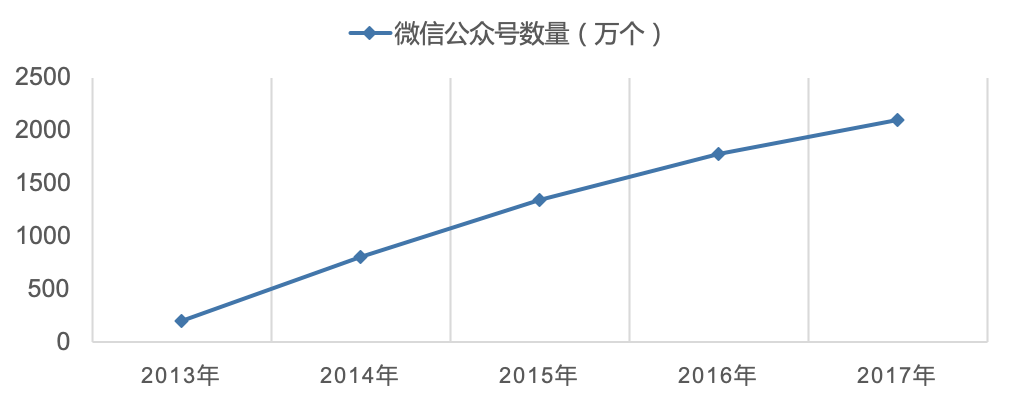
\includegraphics[width=0.9\linewidth]{pub.png}
      \caption{微信公众号数量统计}
      \label{fig:pub}
    \end{figure}

    为顺应该形势,近年来各地政府纷纷开通微信公众号作为官媒的新形式,发挥着宣传渠道、服务平台与展示窗口的关键作用。由此,本文拟采用官方或官方媒体的微信公众号作为官媒的代表进行研究。

    \section{研究问题}
    尽管官媒发布的内容往往是经由工作团队精心挑选或编写的,但受众并非对于官媒发布的所有内容都感到兴趣。换言之,即便在相同的官媒中,发布不同的官媒内容也将呈现出不同的传播效力。

    以目前微信平台上目前最大的官方媒体之一“人民日报”为例,2019年8月19日发布的题为《为了一名高三女孩,末班公交每天多等5分钟,直到她考上大学……》一文,收获了10万以上阅读量,10万以上点赞量;而在2019年8月26日发布的题为《【提醒】微信工作群“说错话”,被公司状告赔偿46万》一文,尽管同样收获了10万以上阅读量,却只有767点赞量。
    
    再以吉林省的官方媒体之一“吉林日报”为例,其平均阅读量和点赞量都远不及“人民日报”。2019年10月9日发布的题为《定了!吉林省这些院校和专业成为省级示范,有你的母校吗?》一文,收获了90906阅读量和302点赞量;而在2019年11月15日发布的题为《动车票低至6.5折、敞开办理团体票业务…吉林车务段推出超多优惠!》一文,却仅收获了670阅读量和3点赞量。
    
    由此两例可见,官媒发布的文本内容同传播效力之间存在一定的联系。本文的目标即为刻画官媒文本内容同该内容传播效力之间的关系,特别地,选取文本内容的主题作为核心特征。

    \section{研究方法}

    \section{数据来源及变量测量}

    \section{研究发现及结果解释}

    \label{applastpage}
    \newpage
    \bibliography{report}
    \bibliographystyle{unsrt}
\iffalse
\begin{itemize}[noitemsep,topsep=0pt]
%no white space
\end{itemize}
\begin{enumerate}[label=\Roman{*}.,noitemsep,topsep=0pt]
%use upper case roman
\end{enumerate}
\begin{multicols}{2}
%two columns
\end{multicols}
\begin{figure}
  \centering
  \includegraphics[width=0.9\linewidth]{}
  \caption{}
  \label{fig:}
\end{figure}
\fi
\end{document}
